\documentclass[11pt,a4paper]{article}
\usepackage[T1]{fontenc}
\usepackage{lmodern}
\usepackage{geometry}
\geometry{margin=23mm}
\usepackage{microtype}
\usepackage{amsmath,amssymb}
\usepackage{booktabs,longtable,array,tabularx}
\usepackage{enumitem}
\usepackage{xcolor}
\usepackage{listings}
\usepackage{tikz}
\usetikzlibrary{arrows.meta,positioning,shapes.geometric,calc,fit}
\usepackage{hyperref}
\usepackage{fancyhdr}
\usepackage{caption}
\usepackage{float}
\usepackage{parskip}

\definecolor{codebg}{RGB}{247,248,250}
\definecolor{codeframe}{RGB}{210,214,220}
\definecolor{commentgreen}{RGB}{0,105,68}
\definecolor{keywordblue}{RGB}{25,70,155}
\definecolor{stringred}{RGB}{150,35,35}

\lstdefinestyle{cstyle}{
  language=C,
  basicstyle=\ttfamily\small,
  keywordstyle=\color{keywordblue}\bfseries,
  commentstyle=\color{commentgreen}\itshape,
  stringstyle=\color{stringred},
  backgroundcolor=\color{codebg},
  frame=single,
  rulecolor=\color{codeframe},
  numbers=left,
  numberstyle=\tiny\color{gray},
  numbersep=8pt,
  showstringspaces=false,
  tabsize=4,
  breaklines=true,
  columns=fullflexible,
  keepspaces=true,
  captionpos=b
}

\setlist[itemize]{topsep=3pt,itemsep=2pt}
\setlist[enumerate]{topsep=3pt,itemsep=3pt}
\setlength{\headheight}{14pt}
\setlength{\parindent}{0pt}
\emergencystretch=2em

\pagestyle{fancy}
\fancyhf{}
\lhead{SmartSafe Project}
\rhead{Timer0, Timer2, and Delay Functions}
\cfoot{\thepage}

\hypersetup{
  colorlinks=true,
  linkcolor=blue!60!black,
  urlcolor=blue!60!black,
  pdftitle={SmartSafe Timer0 Timer2 and Delay Functions},
  pdfauthor={Microprocessors End-Term Project}
}

\title{\textbf{SmartSafe Master and Slave Units}\\[4pt]
\Large Complete Design and Code Explanation of Timer2, Timer0, \texttt{delay\_ms()}, and \texttt{delay\_us()}}
\author{Microprocessors End-Term Project}
\date{July 2026}

\begin{document}
\maketitle
\thispagestyle{empty}

\begin{abstract}
This report documents the timing infrastructure used by the SmartSafe ATmega32 Master and Slave units. Timer2 operates as the continuously running application time base. It is configured in Clear Timer on Compare Match mode to produce a compare event approximately every 10 ms, from which software derives 100 ms service ticks and one-second countdowns. Timer0 is reserved as a temporary, polled timing resource for blocking millisecond and microsecond delays, mainly during LCD initialization and command transfers. The report explains every relevant register, the selected prescalers, the calculations leading to \texttt{OCR2=77}, \texttt{OCR0=124}, and \texttt{OCR0=7}, the write-one-to-clear flag behavior, safe interrupt handling, atomic timestamp reads, Timer2 operation in the Master and Slave, and the limitations of software-polled delays on an 8-bit AVR.
\end{abstract}

\tableofcontents
\newpage

\section{Purpose of the Timing Subsystem}
The SmartSafe program has several activities that must occur at predictable intervals:
\begin{itemize}
  \item the tamper sensor is serviced approximately every 100 ms;
  \item the power comparator stability filter is updated approximately every 10 ms;
  \item the inactivity timer counts toward the 10-second sleep timeout;
  \item the servo remains open for approximately 5 seconds;
  \item a security lockout remains active for approximately 30 seconds;
  \item the Slave keeps LEDs and the alarm active for selected durations;
  \item LCD commands require short delays measured in microseconds or milliseconds.
\end{itemize}

A single timing mechanism is not ideal for all these tasks. The implementation therefore separates the responsibilities:
\begin{enumerate}
  \item \textbf{Timer2} is a background, interrupt-driven system tick. It continues to run while ordinary foreground code executes.
  \item \textbf{Timer0} is temporarily configured for a requested blocking delay. It is polled rather than interrupt-driven, then restored to its earlier state.
\end{enumerate}

Timer1 is not discussed in detail here because it is dedicated to the servo PWM waveform and is documented in the separate servo report.

\section{General Operation of an AVR Timer/Counter}
An AVR timer contains a binary counter register. A selected clock source advances this counter. The clock can be the CPU clock directly or the CPU clock divided by a prescaler.

For a timer clock derived from the CPU clock,
\[
f_{timer}=\frac{F_{CPU}}{N},
\]
where \(N\) is the prescaler. The duration of one timer count is
\[
T_{count}=\frac{N}{F_{CPU}}.
\]

In Clear Timer on Compare Match mode, commonly called CTC mode, the counter starts at zero and increments until its value matches the output compare register. A compare flag is then set, and the counter restarts at zero. Since zero is included, the number of timer counts in one CTC period is
\[
\text{counts}=OCR+1.
\]
Therefore,
\[
T_{CTC}=(OCR+1)\frac{N}{F_{CPU}},
\]
and
\[
f_{CTC}=\frac{F_{CPU}}{N(OCR+1)}.
\]

The project assumes
\[
F_{CPU}=8\,000\,000\text{ Hz}.
\]
The Proteus clock-frequency property of both ATmega32 devices must also be set to 8 MHz. A mismatch between the simulated clock and the compile-time value changes every timer period, the servo waveform, and the USART baud rate.

\section{Timer2 as the Periodic System Tick}
\subsection{Why Timer2 is used}
Timer2 is an 8-bit timer. It is sufficient for generating a short periodic interrupt and leaves Timer1 free for the servo PWM. Timer2 is not used for a long 1-second hardware period directly because an 8-bit counter can represent only 256 counter states. Instead, the hardware produces a period close to 10 ms, and software counts groups of these interrupts.

The selected structure is:
\begin{center}
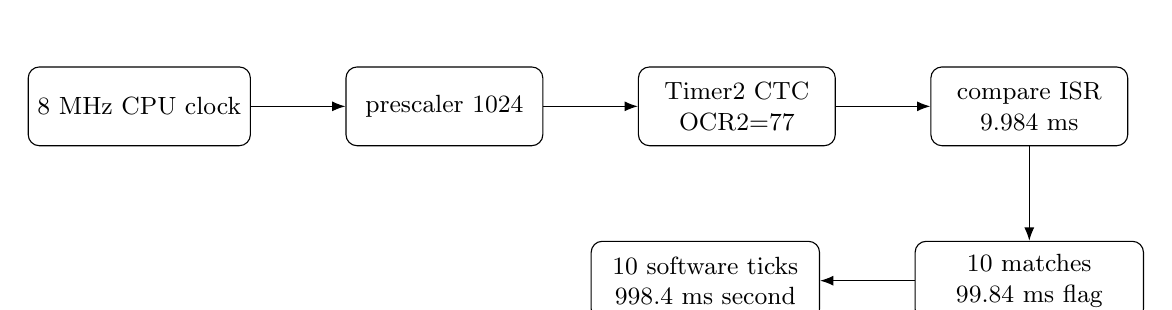
\begin{tikzpicture}[>=Latex,node distance=12mm,every node/.style={font=\small,align=center}]
\node[draw,rounded corners,minimum width=28mm,minimum height=10mm] (clock) {8 MHz CPU clock};
\node[draw,rounded corners,right=of clock,minimum width=25mm,minimum height=10mm] (pre) {prescaler 1024};
\node[draw,rounded corners,right=of pre,minimum width=25mm,minimum height=10mm] (t2) {Timer2 CTC\\OCR2=77};
\node[draw,rounded corners,right=of t2,minimum width=25mm,minimum height=10mm] (irq) {compare ISR\\9.984 ms};
\node[draw,rounded corners,below=of irq,minimum width=29mm,minimum height=10mm] (tick100) {10 matches\\99.84 ms flag};
\node[draw,rounded corners,left=of tick100,minimum width=29mm,minimum height=10mm] (sec) {10 software ticks\\998.4 ms second};
\draw[->] (clock) -- (pre);
\draw[->] (pre) -- (t2);
\draw[->] (t2) -- (irq);
\draw[->] (irq) -- (tick100);
\draw[->] (tick100) -- (sec);
\end{tikzpicture}
\end{center}

\subsection{Timer2 registers}
The relevant ATmega32 registers are:
\begin{center}
\begin{tabularx}{\textwidth}{lX}
\toprule
Register & Role \\
\midrule
\texttt{TCCR2} & Selects Timer2 waveform mode and clock prescaler. \\
\texttt{TCNT2} & Holds the current 8-bit counter value. \\
\texttt{OCR2} & Holds the Timer2 compare value used as TOP in CTC mode. \\
\texttt{TIMSK} & Contains the Timer2 compare-interrupt enable bit \texttt{OCIE2}. \\
\texttt{TIFR} & Contains the Timer2 compare flag \texttt{OCF2}; this flag is cleared by writing a logic one. \\
\texttt{SREG} & Contains the global interrupt-enable bit and is saved while Timer2 is configured atomically. \\
\bottomrule
\end{tabularx}
\end{center}

\subsection{Timer2 initialization code}
The final initialization pattern is:
\begin{lstlisting}[style=cstyle,caption={Timer2 initialization used by the SmartSafe project.}]
void timer2_init(void)
{
    uint8_t saved_sreg = SREG;
    cli();

    TCCR2 = 0;
    TCNT2 = 0;
    OCR2  = 77U;
    TIFR  = (1U << OCF2);

    sub10ms = 0;
    sub100ms = 0;
    timer_tick_100ms = 0;

    TIMSK |= (1U << OCIE2);

    TCCR2 = (1U << WGM21) |
            (1U << CS22)  |
            (1U << CS21)  |
            (1U << CS20);

    SREG = saved_sreg;
}
\end{lstlisting}

\subsection{Why the timer is stopped first}
\begin{lstlisting}[style=cstyle]
TCCR2 = 0;
\end{lstlisting}
With all clock-select bits cleared, Timer2 is stopped. This prevents the counter from advancing while \texttt{TCNT2}, \texttt{OCR2}, flags, and software subcounters are being initialized.

\subsection{Counter reset}
\begin{lstlisting}[style=cstyle]
TCNT2 = 0;
\end{lstlisting}
The counter starts from a known value. Without this assignment, a prior Timer2 state could shorten the first interval.

\subsection{CTC mode selection}
\begin{lstlisting}[style=cstyle]
TCCR2 = (1U << WGM21) | ...;
\end{lstlisting}
The Timer2 waveform-generation bits are:
\begin{center}
\begin{tabular}{ccc}
\toprule
\texttt{WGM21} & \texttt{WGM20} & Mode \\
\midrule
1 & 0 & CTC; clear Timer2 when \texttt{TCNT2=OCR2} \\
\bottomrule
\end{tabular}
\end{center}
No Timer2 output pin is required. The project uses only the compare event and its interrupt.

\subsection{Prescaler selection}
The clock-select bits are:
\begin{center}
\begin{tabular}{cccc}
\toprule
\texttt{CS22} & \texttt{CS21} & \texttt{CS20} & Timer2 clock \\
\midrule
1 & 1 & 1 & \(F_{CPU}/1024\) \\
\bottomrule
\end{tabular}
\end{center}
Thus,
\[
f_{T2}=\frac{8\,000\,000}{1024}=7\,812.5\text{ Hz}.
\]
One Timer2 count takes
\[
T_{count}=\frac{1}{7\,812.5}=128\ \mu\text{s}.
\]

A large prescaler is appropriate because the desired period is close to 10 ms. A smaller prescaler would require more than 256 counts and would not fit in an 8-bit timer.

\subsection{Calculation of OCR2}
For a target period of approximately 10 ms,
\[
OCR2=\frac{F_{CPU}T}{N}-1.
\]
Substituting \(F_{CPU}=8\) MHz, \(T=0.010\) s, and \(N=1024\):
\[
OCR2=\frac{8\,000\,000\times0.010}{1024}-1
=77.125.
\]
The register must hold an integer. The closest convenient value is 77. The actual period is
\[
T_{match}=(77+1)\frac{1024}{8\,000\,000}
=9.984\text{ ms}.
\]
The compare frequency is
\[
f_{match}=\frac{1}{9.984\text{ ms}}
\approx100.1603\text{ Hz}.
\]

The use of \texttt{OCR2=77}, rather than 78, follows from the inclusive count sequence:
\[
0,1,2,\ldots,77.
\]
This sequence contains 78 timer counts.

\subsection{Compare flag and interrupt enable}
\begin{lstlisting}[style=cstyle]
TIFR  = (1U << OCF2);
TIMSK |= (1U << OCIE2);
\end{lstlisting}
\texttt{OCF2} is a write-one-to-clear flag. Assigning a one to this bit removes a stale compare event before interrupts are enabled. This differs from ordinary variables: writing zero does not clear the flag.

Setting \texttt{OCIE2} allows a Timer2 compare match to request the \texttt{TIMER2\_COMP} interrupt. The global interrupt-enable bit in \texttt{SREG} must also be set, normally by \texttt{sei()} after system initialization.

\subsection{Why SREG is saved and restored}
\begin{lstlisting}[style=cstyle]
uint8_t saved_sreg = SREG;
cli();
...
SREG = saved_sreg;
\end{lstlisting}
Timer initialization modifies registers shared with interrupt operation. Disabling interrupts makes the configuration sequence atomic. Restoring the saved \texttt{SREG} value is better than always calling \texttt{sei()}, because the function preserves the interrupt state chosen by its caller.

\section{Timer2 Interrupt Service Routine in the Master}
A representative Master ISR is:
\begin{lstlisting}[style=cstyle,caption={Master Timer2 compare ISR.}]
ISR(TIMER2_COMP_vect)
{
    power_monitor_tick_10ms();

    if (++sub10ms < 10U)
        return;

    sub10ms = 0;
    timer_tick_100ms = 1;

    if (++sub100ms < 10U)
        return;

    sub100ms = 0;
    system_time_s++;

    if (activity_timer < 255U)
        activity_timer++;

    if (lockout_active && lockout_counter > 0U)
        lockout_counter--;

    if (servo_open && servo_counter > 0U)
        servo_counter--;
}
\end{lstlisting}

\subsection{The 10 ms service level}
The power-failure stability filter is serviced on every compare match:
\begin{lstlisting}[style=cstyle]
power_monitor_tick_10ms();
\end{lstlisting}
Each invocation represents approximately 9.984 ms. A confirmation count of ten ticks therefore represents approximately 99.84 ms.

\subsection{The 100 ms service level}
\begin{lstlisting}[style=cstyle]
if (++sub10ms < 10U)
    return;

sub10ms = 0;
timer_tick_100ms = 1;
\end{lstlisting}
Ten Timer2 periods create
\[
10\times9.984=99.84\text{ ms}.
\]
The ISR sets a flag rather than performing ADC conversion or complex application logic inside the interrupt. The main loop sees the flag, clears it, and calls the tamper-processing function.

This keeps the ISR short and reduces interrupt latency. However, the flag is a single bit-like variable. If the main loop remains blocked for more than one 100 ms interval, multiple periodic events can collapse into one pending flag. That behavior is acceptable for the project because the tamper sensor does not require an exact sample count, but it should be understood as a design tradeoff.

\subsection{The one-second service level}
Ten 100 ms software periods produce
\[
10\times99.84=998.4\text{ ms}.
\]
At this boundary, the timestamp and application counters are updated.

The difference from an exact second is
\[
1000-998.4=1.6\text{ ms},
\]
which is a relative error of
\[
\frac{1.6}{1000}\times100=0.16\%.
\]
Therefore the software time base runs approximately 0.16 percent fast. Examples are:
\begin{center}
\begin{tabular}{lcc}
\toprule
Nominal interval & Actual interval from Timer2 & Difference \\
\midrule
5 seconds & 4.992 seconds & -8 ms \\
10 seconds & 9.984 seconds & -16 ms \\
30 seconds & 29.952 seconds & -48 ms \\
\bottomrule
\end{tabular}
\end{center}
This error is negligible for the human-scale lockout, sleep, alarm, and servo durations used in the simulation.

\subsection{Inactivity counter saturation}
\begin{lstlisting}[style=cstyle]
if (activity_timer < 255U)
    activity_timer++;
\end{lstlisting}
The variable is eight bits wide. Saturation at 255 prevents wraparound to zero. Without this check, a system left active for 256 seconds could make the inactivity counter appear newly reset.

\subsection{Countdown counters}
The lockout and servo counters decrement once per software second. The main loop owns the actual state transition. For example, when the servo count reaches zero, foreground code sends the lock command. This separation avoids calling peripheral drivers from inside Timer2's ISR.

\section{Timer2 Operation in the Slave}
The Slave uses the same hardware values:
\begin{lstlisting}[style=cstyle]
OCR2 = 77U;
TCCR2 = (1U << WGM21) |
        (1U << CS22)  |
        (1U << CS21)  |
        (1U << CS20);
\end{lstlisting}

The Slave ISR has fewer responsibilities. It converts 100 Timer2 compare events into one software second and decrements the red-alarm and green-success countdowns:
\begin{lstlisting}[style=cstyle,caption={Simplified Slave Timer2 ISR.}]
ISR(TIMER2_COMP_vect)
{
    if (++sub10ms < 10U)
        return;

    sub10ms = 0;

    if (++sub100ms < 10U)
        return;

    sub100ms = 0;

    if (alarm_counter > 0U)
        alarm_counter--;

    if (green_counter > 0U)
        green_counter--;
}
\end{lstlisting}

The main loop observes the counters and turns outputs off when they reach zero. This makes Timer2 a shared scheduler without placing LCD or buzzer operations inside the interrupt.

\section{Atomic Reading of the 32-bit Timestamp}
The ATmega32 is an 8-bit CPU, while \texttt{system\_time\_s} is a 32-bit value. Reading the variable requires several machine accesses. Timer2 could interrupt between these accesses and increment the value, producing a mixed result.

The safe accessor is:
\begin{lstlisting}[style=cstyle]
uint32_t timer_get_seconds(void)
{
    uint32_t value;
    uint8_t saved_sreg = SREG;

    cli();
    value = system_time_s;
    SREG = saved_sreg;

    return value;
}
\end{lstlisting}

Disabling interrupts for only the short copy guarantees that all four bytes belong to the same timestamp. The original interrupt state is then restored.

\section{Timer0 as a Blocking Delay Generator}
\subsection{Why Timer0 is used separately}
Timer2 must remain configured as the system tick. Reconfiguring Timer2 for an LCD delay would disturb the lockout, tamper, power-filter, and servo timing. Timer0 is therefore used as a temporary timing resource.

The delay functions do not enable a Timer0 interrupt. They poll the compare flag directly:
\begin{center}
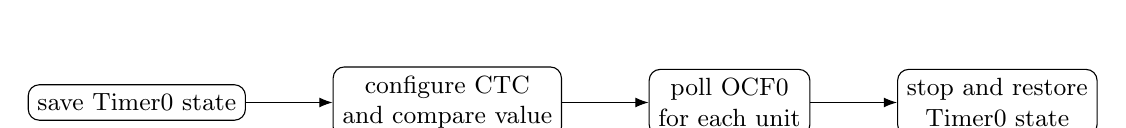
\begin{tikzpicture}[>=Latex,node distance=11mm,every node/.style={font=\small,align=center}]
\node[draw,rounded corners] (save) {save Timer0 state};
\node[draw,rounded corners,right=of save] (cfg) {configure CTC\\and compare value};
\node[draw,rounded corners,right=of cfg] (poll) {poll OCF0\\for each unit};
\node[draw,rounded corners,right=of poll] (restore) {stop and restore\\Timer0 state};
\draw[->] (save) -- (cfg);
\draw[->] (cfg) -- (poll);
\draw[->] (poll) -- (restore);
\end{tikzpicture}
\end{center}

The CPU remains busy inside the delay loop, so these functions are blocking. Global interrupts remain enabled, which means Timer2 can normally continue running while the foreground waits.

\subsection{Timer0 registers}
\begin{center}
\begin{tabularx}{\textwidth}{lX}
\toprule
Register & Role \\
\midrule
\texttt{TCCR0} & Selects Timer0 CTC mode and prescaler. \\
\texttt{TCNT0} & Holds the current Timer0 count. \\
\texttt{OCR0} & Holds the compare value that defines one delay unit. \\
\texttt{TIMSK} & Contains \texttt{OCIE0}; the delay functions disable this interrupt because they poll instead. \\
\texttt{TIFR} & Contains \texttt{OCF0}; writing one clears the compare flag. \\
\bottomrule
\end{tabularx}
\end{center}

\section{Millisecond Delay Function}
\subsection{Correct implementation}
\begin{lstlisting}[style=cstyle,caption={Timer0-based blocking millisecond delay.}]
void delay_ms(uint16_t ms)
{
    uint8_t saved_tccr0 = TCCR0;
    uint8_t saved_timsk = TIMSK;
    uint8_t saved_ocr0  = OCR0;
    uint8_t saved_tcnt0 = TCNT0;

    TCCR0 = 0;
    TIMSK &= ~(1U << OCIE0);

    OCR0  = 124U;
    TCNT0 = 0;
    TIFR  = (1U << OCF0);

    TCCR0 = (1U << WGM01) |
            (1U << CS01)  |
            (1U << CS00);

    while (ms-- > 0U) {
        TCNT0 = 0;
        TIFR = (1U << OCF0);

        while (!(TIFR & (1U << OCF0))) {
            /* blocking wait */
        }
    }

    TCCR0 = 0;
    TIFR = (1U << OCF0);
    OCR0 = saved_ocr0;
    TCNT0 = saved_tcnt0;
    TIMSK = saved_timsk;
    TCCR0 = saved_tccr0;
}
\end{lstlisting}

\subsection{Timer0 CTC mode}
For Timer0,
\begin{center}
\begin{tabular}{ccc}
\toprule
\texttt{WGM01} & \texttt{WGM00} & Mode \\
\midrule
1 & 0 & CTC using \texttt{OCR0} \\
\bottomrule
\end{tabular}
\end{center}
The project does not use the OC0 output pin. It only waits for the internal compare flag.

\subsection{Prescaler and OCR0 calculation}
The millisecond function selects a prescaler of 64:
\begin{center}
\begin{tabular}{cccc}
\toprule
\texttt{CS02} & \texttt{CS01} & \texttt{CS00} & Timer0 clock \\
\midrule
0 & 1 & 1 & \(F_{CPU}/64\) \\
\bottomrule
\end{tabular}
\end{center}
Thus,
\[
f_{T0}=\frac{8\,000\,000}{64}=125\,000\text{ Hz}.
\]
One count takes
\[
T_{count}=\frac{1}{125\,000}=8\ \mu\text{s}.
\]
The number of counts required for 1 ms is
\[
\frac{1\text{ ms}}{8\ \mu\text{s}}=125.
\]
Since the timer counts from zero through the compare value,
\[
OCR0=125-1=124.
\]
The ideal hardware compare interval is therefore
\[
(124+1)\times8\ \mu\text{s}=1000\ \mu\text{s}=1\text{ ms}.
\]

\subsection{Why OCIE0 is disabled}
\begin{lstlisting}[style=cstyle]
TIMSK &= ~(1U << OCIE0);
\end{lstlisting}
The function waits for \texttt{OCF0} itself. Enabling the Timer0 compare interrupt would be unnecessary and could invoke an unrelated ISR. Only the Timer0 interrupt-enable bit is changed; the saved \texttt{TIMSK} value is restored afterward.

\subsection{Why the flag is cleared before each interval}
\begin{lstlisting}[style=cstyle]
TIFR = (1U << OCF0);
\end{lstlisting}
A previous compare may have left \texttt{OCF0=1}. If the stale flag were not cleared, the polling loop could terminate immediately and produce a zero-length interval. The ATmega32 clears this flag by writing a logic one.

\subsection{Why TCNT0 is reset each time}
\begin{lstlisting}[style=cstyle]
TCNT0 = 0;
\end{lstlisting}
Resetting the counter establishes a complete 125-count interval for each requested millisecond. It also makes the function independent of the count value that existed before the current loop iteration.

\subsection{Accuracy of \texttt{delay\_ms()}}
The timer portion of each iteration is exactly 1 ms for an ideal 8 MHz CPU clock. The complete function is slightly longer because software executes loop control, register writes, and the polling branch. Therefore,
\[
T_{actual}\gtrsim ms\times1\text{ ms}.
\]
The overhead is small compared with a millisecond and is acceptable for LCD power-up, clear-display, and human-interface pauses. It should not be treated as a laboratory-grade time reference.

\section{Microsecond Delay Function}
\subsection{Corrected robust implementation}
The reliable final implementation uses the full 8 MHz Timer0 clock and eight timer counts for each nominal microsecond:
\begin{lstlisting}[style=cstyle,caption={Corrected Timer0-based microsecond delay.}]
void delay_us(uint16_t us)
{
    uint8_t saved_tccr0 = TCCR0;
    uint8_t saved_timsk = TIMSK;
    uint8_t saved_ocr0  = OCR0;
    uint8_t saved_tcnt0 = TCNT0;

    TCCR0 = 0;
    TIMSK &= ~(1U << OCIE0);

    OCR0  = 7U;
    TCNT0 = 0;
    TIFR  = (1U << OCF0);

    TCCR0 = (1U << WGM01) |
            (1U << CS00);

    while (us-- > 0U) {
        TCNT0 = 0;
        TIFR = (1U << OCF0);

        while (!(TIFR & (1U << OCF0))) {
            /* blocking wait */
        }
    }

    TCCR0 = 0;
    TIFR = (1U << OCF0);
    OCR0 = saved_ocr0;
    TCNT0 = saved_tcnt0;
    TIMSK = saved_timsk;
    TCCR0 = saved_tccr0;
}
\end{lstlisting}

\subsection{No-prescaler calculation}
With \texttt{CS00=1} and the other clock-select bits zero,
\[
f_{T0}=F_{CPU}=8\,000\,000\text{ Hz}.
\]
One timer count is
\[
T_{count}=\frac{1}{8\,000\,000}=0.125\ \mu\text{s}.
\]
Eight counts produce
\[
8\times0.125\ \mu\text{s}=1\ \mu\text{s}.
\]
Since CTC counts from zero through \texttt{OCR0},
\[
OCR0=8-1=7.
\]
Thus, the hardware comparison interval is nominally 1 microsecond.

\subsection{Why the earlier OCR0=0 form was replaced}
An earlier version selected a prescaler of 8 and used \texttt{OCR0=0}. Mathematically, one divided timer count equals 1 microsecond at 8 MHz. However, a zero compare value creates an extremely short compare sequence and behaved unreliably in the Proteus simulation used for this project. The LCD initialization could stall while waiting for a flag transition.

The corrected form uses eight physical counter states at the undivided clock:
\begin{lstlisting}[style=cstyle]
OCR0 = 7U;
TCCR0 = (1U << WGM01) | (1U << CS00);
\end{lstlisting}
This represents the same ideal microsecond duration but provides a clearer and more robust simulated timer interval.

\subsection{Accuracy limitation at very short delays}
For \texttt{delay\_us(1)}, software overhead is comparable to or greater than the requested timer interval. Register writes, loop branches, and function call/return instructions all consume CPU cycles. Therefore the function guarantees a safe minimum delay rather than an exact one-microsecond wall-clock interval:
\[
T_{actual}>1\ \mu\text{s}\quad\text{for very small arguments}.
\]
This is appropriate for the HD44780-compatible LCD, where delays must be at least a specified minimum. It is not appropriate for generating a high-precision communication waveform. Hardware PWM, SPI, USART, or output compare should be used for exact high-speed signaling.

\section{Saving and Restoring Timer0 State}
Both delay functions save:
\begin{lstlisting}[style=cstyle]
TCCR0, TIMSK, OCR0, TCNT0
\end{lstlisting}
This allows Timer0 to be borrowed without permanently destroying a configuration established elsewhere.

The restoration order is deliberate:
\begin{enumerate}
  \item set \texttt{TCCR0=0} to stop Timer0;
  \item clear the final compare flag;
  \item restore \texttt{OCR0} and \texttt{TCNT0};
  \item restore \texttt{TIMSK};
  \item restore \texttt{TCCR0} last, so the previous clock starts only after all associated state is ready.
\end{enumerate}

The functions do not save \texttt{TIFR}, because interrupt flags are event indicators rather than ordinary configuration state. The delay clears its own compare event before returning.

\section{Interaction Between Timer0 Delays and Timer2}
Timer0 polling blocks the foreground code, but it does not call \texttt{cli()}. Therefore Timer2 interrupts remain enabled and continue to update system timing during most delay calls.

For example, during a 1.5-second LCD splash delay:
\begin{itemize}
  \item Timer0 repeatedly generates the millisecond wait intervals;
  \item Timer2 still interrupts approximately every 9.984 ms;
  \item the application timestamp and inactivity counter continue to advance;
  \item the foreground cannot scan the keypad or service a one-bit 100 ms flag until the delay returns.
\end{itemize}

This is why blocking delays should be kept short during normal operation. Long human-scale behaviors, such as the 5-second servo interval and 30-second lockout, are implemented with Timer2 counters rather than \texttt{delay\_ms()}.

\section{Timer Behavior During Sleep and Power Standby}
Timer operation depends on the selected AVR sleep mode and on whether the firmware explicitly stops a timer.

In ordinary inactivity Power-down sleep, synchronous timers driven from the CPU clock stop. Timer2 therefore does not count the sleep duration in the current design. The external interrupt on \texttt{INT0} wakes the Master, after which normal timing resumes.

During power-failure standby, the firmware preserves the analog comparator as the restoration wake source and may disable ordinary runtime peripherals, including Timer2. The comparator transition wakes the CPU, the power module accepts restoration, and the runtime initialization restores Timer2.

The blocking Timer0 functions must not be called while the CPU is already sleeping. They require a running CPU clock because the foreground actively polls \texttt{OCF0}.

\section{Why Long Delays Are Not Implemented with Timer0}
A call such as
\begin{lstlisting}[style=cstyle]
delay_ms(30000U);
\end{lstlisting}
would block the main loop for 30 seconds. During that interval, the system could not process keypad input, USART commands, state transitions, or ordinary foreground events. Although Timer2 interrupts might continue, the architecture would become unresponsive.

The project instead uses nonblocking application counters:
\begin{lstlisting}[style=cstyle]
lockout_counter = 30U;
servo_counter   = 5U;
\end{lstlisting}
Timer2 decrements them in the background while the main loop remains available for other work.

The design rule is:
\begin{center}
\begin{tabular}{ll}
\toprule
Timing requirement & Mechanism \\
\midrule
LCD setup and bus timing & Timer0 blocking delay \\
Short initialization pause & Timer0 blocking delay \\
Periodic 10 ms and 100 ms service & Timer2 interrupt \\
5-second servo interval & Timer2 software countdown \\
10-second inactivity interval & Timer2 software counter \\
30-second lockout or breach alarm & Timer2 software countdown \\
Precise servo pulse train & Timer1 hardware PWM \\
\bottomrule
\end{tabular}
\end{center}

\section{Common Errors and Their Symptoms}
\begin{longtable}{p{0.29\textwidth}p{0.31\textwidth}p{0.31\textwidth}}
\toprule
Error & Consequence & Correction \\
\midrule
Proteus MCU clock left at 1 MHz & All timer intervals become approximately eight times too long; USART and servo also fail & Set both ATmega32 clock properties to 8 MHz \\
Forgetting the \(+1\) in CTC calculations & Compare periods are off by one timer count & Use \(T=(OCR+1)N/F_{CPU}\) \\
Clearing \texttt{OCF0} or \texttt{OCF2} by writing zero & Stale flag remains set & Clear by writing a logic one \\
Using \texttt{OCR0=0} for the microsecond delay in Proteus & Possible simulation stall or unreliable LCD timing & Use no prescaler and \texttt{OCR0=7} \\
Not resetting \texttt{TCNT0} & First delay interval can be shortened & Set \texttt{TCNT0=0} for each unit \\
Reconfiguring Timer2 for a delay & System tick and countdowns are corrupted & Reserve Timer2 for periodic scheduling and use Timer0 for delays \\
Using a long blocking delay for lockout & Keypad, USART, and main-loop processing freeze & Use Timer2 countdown variables \\
Reading \texttt{system\_time\_s} without atomic protection & A mixed 32-bit timestamp may be obtained & Use \texttt{timer\_get\_seconds()} \\
Leaving \texttt{OCIE0} enabled while polling & An unwanted Timer0 ISR may run & Temporarily clear \texttt{OCIE0} and restore \texttt{TIMSK} later \\
Restoring Timer0 clock before its compare/count values & Previous timer configuration can run briefly with wrong state & Restore \texttt{TCCR0} last \\
\bottomrule
\end{longtable}

\section{Proteus Verification Procedure}
\subsection{Timer2}
A practical verification method is to toggle an unused debug pin in the Timer2 ISR and observe it with the Proteus oscilloscope or logic analyzer. Toggling on every compare produces a square wave whose half-period is approximately 9.984 ms and full period is approximately 19.968 ms. Setting a pin high for one ISR and low for the next can also reveal the interrupt interval.

The 100 ms flag can be tested by toggling another pin only when \texttt{sub10ms} reaches ten. The observed event spacing should be approximately 99.84 ms.

\subsection{\texttt{delay\_ms()}}
Set a debug output high, call \texttt{delay\_ms(100)}, then set it low. The high pulse should be slightly longer than 100 ms because of software overhead.

\subsection{\texttt{delay\_us()}}
For a visible logic-analyzer test, use a larger argument such as \texttt{delay\_us(100)}. Very short calls are dominated by software overhead and simulation resolution. The function is intended to satisfy minimum LCD timing, not to serve as a calibrated pulse generator.

\section{Design Summary}
Timer2 is the SmartSafe scheduler. With an 8 MHz CPU clock, prescaler 1024, CTC mode, and \texttt{OCR2=77}, it produces a 9.984 ms compare event. Software groups ten events into a 99.84 ms service flag and ten of those groups into a 998.4 ms application second. This supplies the power confirmation filter, tamper service flag, timestamps, sleep timeout, servo interval, lockout, and Slave indicator countdowns.

Timer0 is a temporary blocking delay resource. For milliseconds, prescaler 64 and \texttt{OCR0=124} create an ideal 1 ms compare interval. For microseconds, the corrected implementation uses no prescaler and \texttt{OCR0=7}, producing an ideal one-microsecond hardware interval from eight 0.125-microsecond counts. Both functions poll \texttt{OCF0}, preserve the previous Timer0 configuration, and restore the timer safely after use.

The central design principle is separation of timing roles: Timer0 handles short blocking hardware delays, Timer2 handles responsive application scheduling, and Timer1 independently generates the servo PWM waveform.

\section*{References}
\addcontentsline{toc}{section}{References}
\begin{enumerate}
  \item Microchip Technology Inc., \textit{ATmega32A Data Sheet}, DS40002072A. \href{https://ww1.microchip.com/downloads/en/DeviceDoc/Atmega32A-DataSheet-Complete-DS40002072A.pdf}{Official Microchip PDF}.
  \item Microchip Technology Inc., \textit{AVR Instruction Set Manual}, DS40002198A. \href{https://ww1.microchip.com/downloads/en/DeviceDoc/AVR-Instruction-Set-Manual-DS40002198A.pdf}{Official Microchip PDF}.
  \item SmartSafe project source files: \texttt{timer.c}, \texttt{timer.h}, \texttt{config.h}, and the Master/Slave main-loop modules.
\end{enumerate}

\end{document}
